\documentclass[twocolumn,linenumbers]{aastex631}
%%\documentclass[linenumbers]{aastex631}
%%\documentclass[modern]{aastex631}
%%\documentclass[twocolumn]{aastex631}
\newcommand{\vdag}{(v)^\dagger}
\newcommand\aastex{AAS\TeX}
\newcommand\latex{La\TeX}

\usepackage{mathtools, graphicx, booktabs, apjfonts, soul}
%\addbibresource{Bibliography.bib} %For bibliography

\begin{document}

\title{Comparison of Titan's Equatorial Landscapes to an Improved Radiative Transfer Model
\footnote{Feb, 26, 2025}}

\author[0000-0002-8482-4669]{Gabriel M Steward}
\affiliation{University of Idaho, Moscow, Idaho 83844}

\author{Jason W. Barnes}
\affiliation{University of Idaho, Moscow, Idaho 83844}

\author{William Miller}
\affiliation{University of Idaho, Moscow, Idaho 83844}

\author{Shannon MacKenzie}
\affiliation{Johns Hopkins University Applied Physics Laboratory, Laurel, Maryland 20723}

\author{Others?}

\begin{abstract}

\textbf{\color{red}NOTE: Red notes are important! Do not submit the document with any of them remaining!\color{black}}

\textbf{\color{blue}NOTE: Blue notes are placeholders! Do not submit the document with any of them remaining!\color{black}}

\textbf{\color{red}ABSTRACTION: this will be done last, as we need to know the end from the beginning to properly do it.\color{black}}

\end{abstract}

\keywords{KEYWORDS (111) --- KEYWORDS (112)}

\section{Introduction} \label{sec:intro}

Titan has one of the least understood surfaces in the entire Solar System, due largely to its thick haze-filled atmosphere that is opaque to most light. While there do exist a handful of atmospheric ``windows'' through which specific wavelengths of light can pass through relatively unimpeded \citep{Barnes2007}, this only allows for tiny slivers of information to be gleaned from the surface. Even within the windows, the thick atmosphere contaminates the relatively small amount of surface information we do receive; transmission is never perfect \citep{EsSayeh2023}. 

To combat this, we turn to radiative transfer models of Titan's atmosphere that predict the influence the atmosphere has on the received signal, allowing for true surface effects to be identified. Many such models have been created over the years, each with their own strengths and weaknesses (\cite{Griffith2012, Xu2013, Barnes2018, Corlies2021, Rannou2021}; and \cite{EsSayeh2023}, to name a few). These radiative transfer models depend on accurate knowledge of Titan's atmosphere, which is most well characterized at the moon's equatorial regions since that is where the Huygens lander measured the atmosphere \citep{Tomasko2008}. Many surface characterizaiton studies attempting to filter out the influence of the atmosphere have been performed in the past \citep{Buratti2006, Soderblom2009, Kazeminejad2011, Brossier2018, EsSayeh2023, Solomonidou2024}. However, the majority of them make a notable assumption: that the surface behaves as lambertian; a perfect scatterer with no directly reflected components. \cite{Buratti2006} is a notable exception. The lambertian assumption is somewhat reasonable for the equatorial regions, as the highly reflective lakes and seas of Titan are restricted to the poles \citep{Hayes2016}. However, the prevalence of opposition surges throughout the Solar System casts doubt on this assumption \citep{Deau2009}. In this paper, we seek to demonstrate the degree to which Titan's equatorial surface terrains exhibit non-lambertian behavior. We compare a lambertian simulation of Titan with real observations; identifying notable differences between the major terrain types in the meantime.

Thye vast majority of observations of Titan's surface have been done by spacecraft visiting Saturn, with the most high-quality data coming from the Cassini mission. As such, many images of Titan's surface are taken at unusual viewing geometries. This is quite useful, as it allows characterization of Titan's surface from most if not all orientations, making it far easier to determine exactly how non-lambertian various terrains are. Many non-lambertian effects, such as the opposition surge \citep{Deau2009} and forward-scattering behavior, are most noticable at extreme viewing angles. Unfortunately, most current radiative transfer models applicable to Titan either assume a plane parallel atmosphere in their calculations \citep{Griffith2012, EsSayeh2023}, don't consider angle at all \citep{Rannou2021}, or use a spherical approximation \citep{Corlies2021}. Thus, all these lose accuracy the further the viewing geometry is from ideal, which is precisely where we wish to look. To gain the useful information contained within observations at non-ideal viewing gometries, the spherical nature of Titan's atmosphere must be considered. Thus, to create our lambertian models, we use SRTC++ (Spherical Radiative Transfer in C++), a radiative transfer code tailored to model Titan in full spherical geometry at the infrared wavelengths available to Cassini's VIMS (Visual and Infrared Mapping Spectrometer) instrument \citep{Barnes2018}. Other spherical models do exist \citep{Xu2013}, but SRTC++ was chosen due to familiarity with the code.

Equipped with a spherical radiative transfer model and atmospheric characterization from Huygens, it is now possible to compare models with reality on a scale covering the entire Cassini mission. As the equatorial regions are the best characterized atmospherically, we choose to examine the dunes, equatorial plains, western Xanadu, and the Huygens Landing Site (HLS) across all viewing geometries with observations of sufficient quality. This analysis serves dual purposes--to qualitatively validate the SRTC++ simulation against real data, and to identify deviations from lambertian behavior on Titan's surface. To accomplish this, first we outline improvments made to SRTC++ in \textbf{Model Methods} and report on those changes in \textbf{Model Results}. We describe the procedure by which we gathered our Titan data in \textbf{Observations and Data}, compare reality to simulation in \textbf{Model vs Data Comparison}, and end with the \textbf{Conclusion}.

\textbf{\color{red}NOTE: Be sure to redo this last introduction paragraph when the paper is done to match the final outline.\color{black}}

\section{Model Methods} \label{sec:model}

\textbf{\color{blue}METHODS: Jason's Section. Brief summary of SRTC++, citing the previous paper for more details. Describe new SRTC++ modules used, notably Abosrption and the switch to Doose atmosphere. There should be a comparison figure to note the differences between the two. Mention the new integration method.\color{black}}

\textbf{\color{blue}Figs: comparison between SRTC++ versions.\color{black}}

\textbf{\color{blue}Will be done by Jason \color{black}}

\section{Model Results} \label{sec:mresults}

\textbf{\color{blue}Can't fully write out this section as it depends heavily on the previous section. So, instead, have a more detailed outline with some potential figures: \color{black}}

\textbf{\color{blue}1) Description of setup; what parameters did we put into SRTC++ to get the simulation results we use and why. Figure 1 shows this arrangement. This paragraph MAY go in the above section (Model Methods), depending on the flow of this paper and what exactly is compared in that section. \color{black}}

\begin{figure}[htbp]
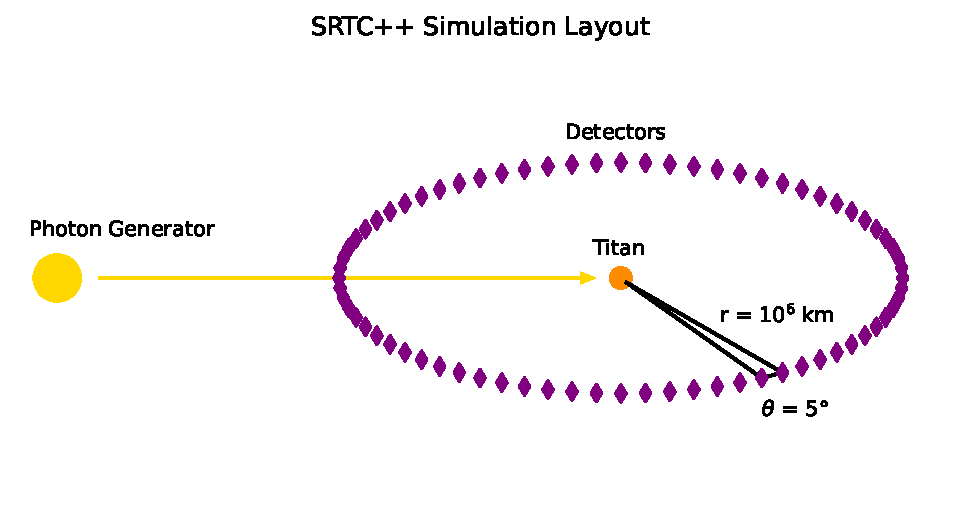
\includegraphics[scale = 0.5]{SRTCLayout.pdf}
\centering
\caption{\textbf{\color{red}NOT FINAL\color{black}} Layout of our SRTC++ simulations. Distances not to scale. Detectors all equidistant from Titan and angular separation is the same for each one. The yellow arrow represents "photon packets" being shot at Titan. Note that it does not interact with the detector it passes through.}
\label{fig:1}
\end{figure}

\textbf{\color{blue}2) The primary figures in this section are Figures 2-4, titancolor2 views of Titan at multiple angles, each at a different albedo. Discuss the lambertian features showing up as they are expected to, and explain the coloration; thankfully it is green now so the awkward blue image is no longer an issue. Discuss the different albedo simulations and the patterns between them. Draw attention to the predictable behavior. Also draw attention to the fact that the pure atmosphere view (180) shows no real difference between the albedos. Note 0.1 albedo as the most Titan-like, visually.\color{black}}

\begin{figure}[htbp]
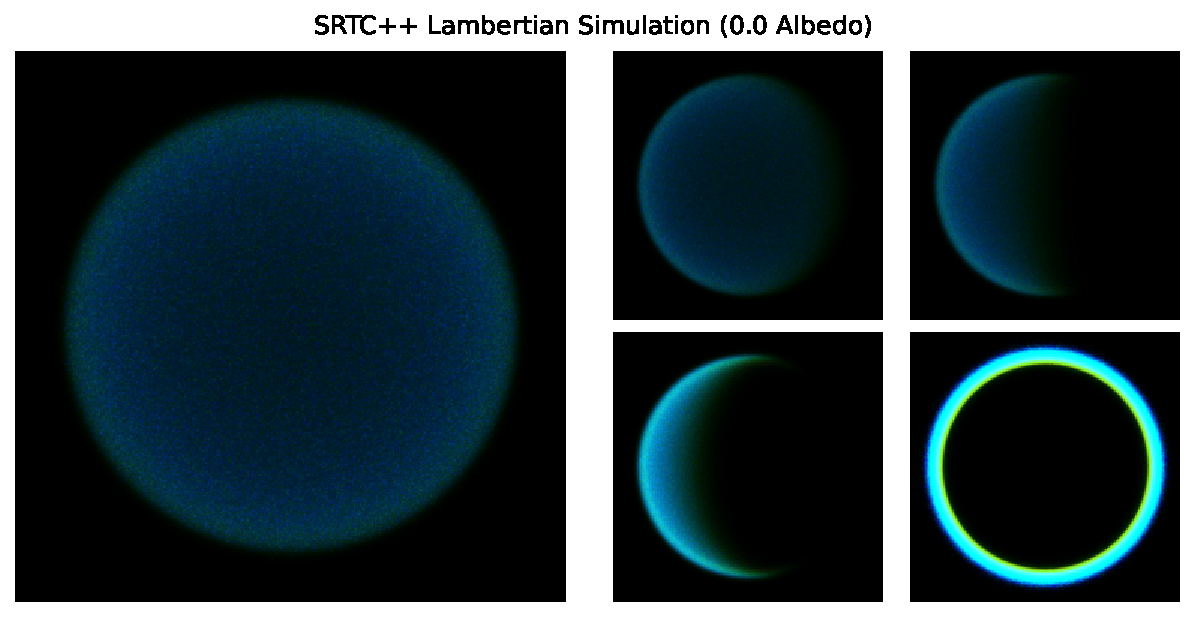
\includegraphics[scale = 0.4]{LambertianSimA0.pdf}
\centering
\caption{\textbf{\color{red} NOT FINAL \color{black}}Simulation results for a lambertian Titan with 0.0 albedo, colored with 5, 2 and 1.3 $\mu$m mapped to red, green, and blue respectively. Left image is viewed at 0$^{\circ}$  from the incidence angle. Right four images are at  35$^{\circ}$, 90$^{\circ}$, 120$^{\circ}$, and 180$^{\circ}$ in left to right then top to bottom order. \textbf{\color{red}[An animating version of the figure will exist in places that support it. The large left panel will hold the animating image, the right panels will remain static for comparisons] \color{black}}}
\label{fig:2}
\end{figure}

\begin{figure}[htbp]
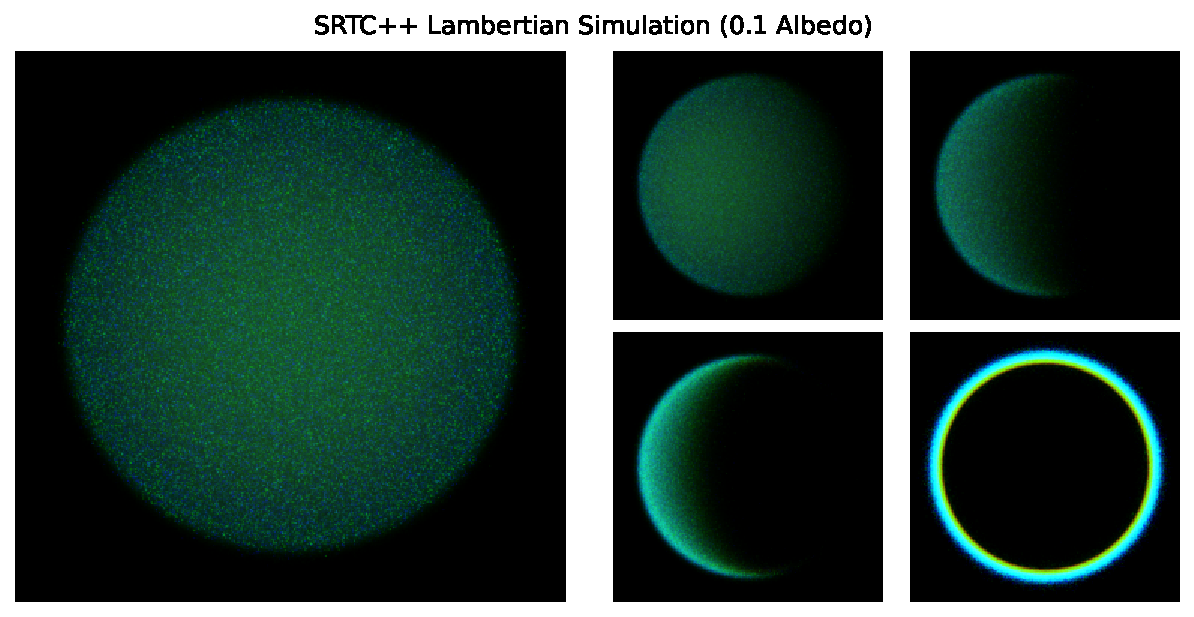
\includegraphics[scale = 0.4]{LambertianSim.pdf}
\centering
\caption{\textbf{\color{red} NOT FINAL \color{black}}Same as Figure 2 but for 0.1 Albedo.}
\label{fig:3}
\end{figure}

\begin{figure}[htbp]
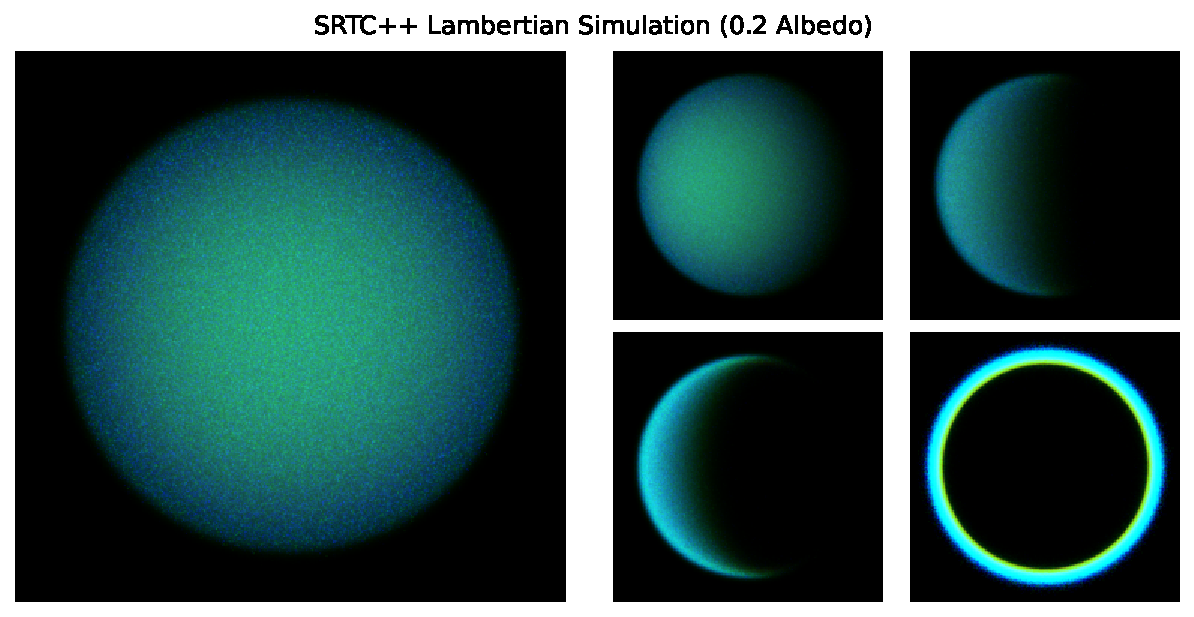
\includegraphics[scale = 0.4]{LambertianSimA2.pdf}
\centering
\caption{\textbf{\color{red} NOT FINAL \color{black}}Same as Figure 2 but for 0.2 Albedo.}
\label{fig:4}
\end{figure}

\textbf{\color{blue}3) Mention that the simulation does other wavelengths as well, but we only focus on these three, and later on just 2 microns. This is to keep the data from being overcrowded. (And to avoid looking at 0.93 but that doesn't need to be mentioned). \color{black}}
 
 \textbf{\color{blue}4) Additional things to possibly address: limb effects, terminator effects, the S/N of the results, more details about why 5um is so weird... \color{black}}

\textbf{\color{blue}5) MAYBE: discuss the viewing angle models. This may not be necessary as the exact setup for these models is described in the Observations and Data section. However, we may wish to use a graph from those models in this section to compare between different albedos, which would belong here and necessitate discussion of the models. If so, this would be a good palce for a figure that shows, visually, the viewing angles. Said figure is Figure 5, which will either be used here or in Observations and Data.\color{black}}

\begin{figure}[htbp]
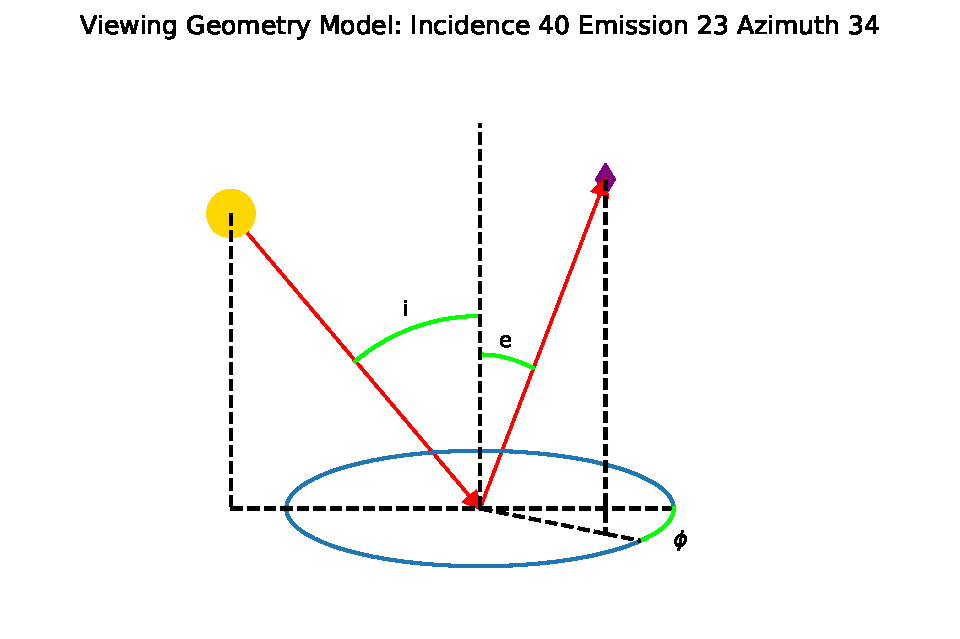
\includegraphics[scale = 0.55]{VGDisplayLabel.pdf}
\centering
\caption{\textbf{\color{red} NOT FINAL \color{black}} Viewing Geometry Angles used in this paper. Incidence angle is represented by ``i'', emission angle by ``e'', and azimuth angle by ``$\phi$.'' The red arrows trace out a path from the sun (yellow circle) to some arbitrary spot on Titan's surface to a detector (purple diamond). \textbf{\color{red} Code exists to make versions of this figure for specific slices of viewing goeometry that can be put on other plots as needed. The other versions will not have the labels, as they'd just get in the way on smaller versions.\color{black}}}
\label{fig:5}
\end{figure}

\section{Observations and Data} \label{sec:observe}

Cassini performed over a hundred separate flybys of Titan during its mission \citep{Seal2017}, and most of those flybys have observaitons from VIMS. Viewing geometries on any single flyby are genreally limited in scope, as the spacecraft itself could only examine geometries it personally encountered. Thus, in order to gain a proper understanding of the surface of Titan at all viewing angles, observations from as many flybys as possible should be used. 

The primary obstacle in properly using all the data is the sheer amount in play; over a hunded flybys, tens of thousands of individual observations, and in each of those hundreds of spectels each with hundreds more individual values associated with them. If we wished to make a single global model, this would not be an issue, as an algorithm could easily ingest everything. However, we desire a different model for every major terrain type on Titan's equatorial surface so that reasonable comparisons can be made between them. To that end, we have created a raster mask of Titan's surface \textbf{\color{blue}(Figure 6)\color{black}}.

\begin{figure}[htbp]
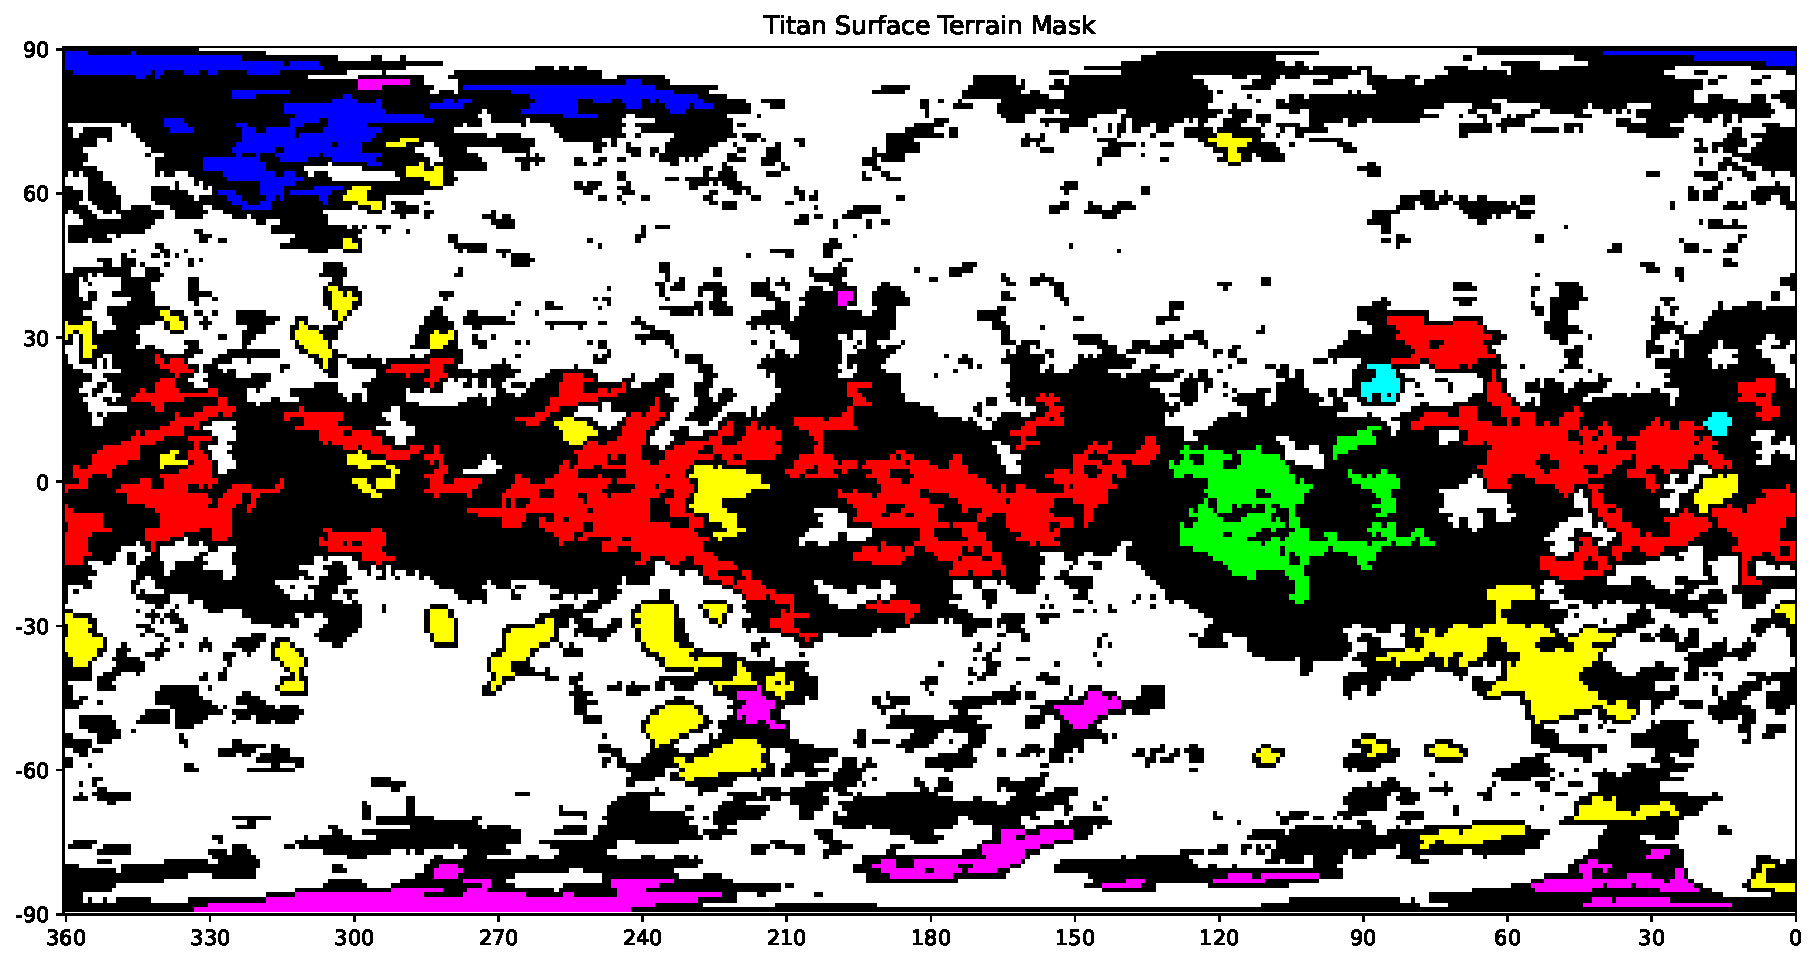
\includegraphics[scale = 0.25]{TitanSurfaceMask.pdf}
\centering
\caption{\textbf{\color{red} NOT FINAL \color{black}} Titan surface terrain mask, as informed by \cite{Lopes2020} mixed with VIMS observations. Black areas are ``Null'' pixels as outlined in the text. White corresponds to ``plains'', red with dunes, yellow with ``hummocky'', blue with lakes and seas, pink with ``labyrinth'' terrain, and green with Xanadu, primarily Western Xanadu. Cyan notes major craters, though this is largely a vestigal feature from \cite{Lopes2020}'s original map. In this work, we only concern ourselves with terrain within thirty degrees latitude from the equator, which ignores ``labyrinth'' terrain and the seas.}
\label{fig:6}
\end{figure}

The creation of the mask began with the Titan terrain map created by \cite{Lopes2020} using radar data. VIMS observations, which are taken in infrared, often don't match the radar observations \citep{Soderblom2007}, but tend to agree in the bulk of major features; most notably (and importantly for this paper) the dunes have good agreement on a global scale.

The resolution in question for the mask is one pixel per degree on Titan's surface; 181 in latitude and 360 in longitude. The radar map was scaled down to reduce it to this resolution. Any pixel that was not clearly or nearly a solid color was replaced with a ``Null'' pixel; one where we would not harvest data from when using the mask to identify terrain. We erred on the side of caution, more likely to assign ``Null'' to a pixel than not. Any pixels of different terrains that were touching were makred ``Null'' as well to avoid contamination. After this we manually removed some areas that notably did not match VIMS data, were too small to be of use, or were known to have different spectral characteristics than other terrains given the same classification. Hotei Regio, Tui Regio, the northern lake district, and Southern Xanadu were notable manual exclusions. Xanadu was deemed large enough not to exclude, but rather to include as its own unique terrain type, due to its known bizarre character \citep{Brown2011}. Notably the part of Xanadu marked as sharing a terrian type consists mostly of Western Xanadu.

In addition to the terrain classification marked by color in \textbf{\color{blue}Figure 6\color{black}} the mask also has a version with a hidden data point: each pixel records its distance to the nearest ``Null'' pixel in km along Titan's surface. This allows the mask to be refined: pixels that are close to ``Null'' pixels can be excluded as likely to have contamination from pointing errors in the VIMS data, which are known to occur \citep{Barnes2008}. 

VIMS observations come in the form of ``cube'' files. Our investion procedure for these files begins with a basic database search; in our specific case, looking for any cubs that have spectels in the equatorial regions between 30 and -30 latitude, and also have spectels of 25 km ground resolution or lower. The database we are using has already filtered out clearly erroneous files, as well as so called ``noodles'' images which are only a handful of spectels in diameter. Once the cubes are identified, they are ingested and each spectel examined to see if it is satisfactory according to provided position, flyby number, or resolution restrictions. If a spectel passes the test, it is added to a list. This list can be made with or without refering to the mask. 

When the mask is used, only spectels marked with a terrain other than ``Null'' are cataloged. In addition to the standard limitations, the spectels can be judged based on their proximity to a ``Null'' pixel on the mask. Two options exist for this: setting a minimum distance from a ``Null'' pixel that will be accepted, or setting an allowed maximum ratio of ground resolution to ``Null'' pixel distance.

When the mask is not used, ``Null'' values can be accepted. This is helpful when wanting to look at areas in or near ``Null'' pixels, such as the Huygens Landing Site. 

To turn the list of spectels into a model, we sort them by their viewing geometries; that is, their incidence, emission, and azimuth angles.  \textbf{\color{red}Alternative placement for Figure 5\color{black}} Every five degrees \textbf{\color{red}(may be changed to ten)\color{black}} marks a bin where the I/F (observed intensity over solar flux) of every spectel is averaged. In the end, we have a model that can take an incidence, emission, and azimuth angle as input while outputting the average I/F found at those geometries. The simulations created with SRTC++ are processed and placed into identically structured viewing gometry models.

There are a few limitaitons to these models. The primary limitation is that certain viewing angles, usually at the extreme ends of allowed values, simply do not exist since Cassini was never in those positions. For terrain types that are expansive and easily seen from basically anywhere, this is hardly a problem, but for somewhat localized areas like Xanadu there are large sections of the model that simply have no data. Particuarly high resolution cubes can reveal small details not visible in most views and thus are not reflected in the mask. These small details need not match the behavior of the terrain they are surrounded by, and could conceivably offset the final model. Again, for larger models, situations like this are likely to be shrouded by the sheer number of data points available, but smaller areas can easily be contaminated. There is also no check for interfering clouds at this time. 

For our global models, we did not change the position and resolution restrictions of the original database search, but did have a minimum ``Null'' distance of 50 km and a maximum ratio of ground resolution to ``Null'' pixel distance of 1/4. \textbf{\color{red}It is somewhat likely that these numbers will change once I figure out what the best numbers ARE.\color{black}}  Each major terrain type was then catalogued into its own individual model, though we do not examine all of them here. 

In addition to the equatorial terrain models, we also made a model for the Huygens Landing Site, as our atmosphere models ultimately draw from observations made by the Huygens lander \citep{Tomasko2008}. We performed a database search similarly to how we made the other models, but we also went in manually afterward, cleaning up any situations where Cassini reported the wrong latitude and longitude for the spectels, ensuring that the data was devoid of any contamination; something we only had to do since the Huygens Landing Site was such a small area. 

\textbf{\color{red}Consider adding section where we justify HLS procedure even further, perhaps noting how many pixels are gathered in each location?\color{black}} 

\section{Model vs Data Comparison} \label{sec:compare}

\textbf{\color{blue}Requres actual results to do this section. We need to decide what we want to show, and how, and I need to figure out what the best parameters are for sifting through the database (which is my current next major step for this research). But we can construct a general outline. There will be two major sections: examination of the Huygens Landing Site and examinations of Equatorial Terrain. \color{black}}

\textbf{\color{blue}1) The Huygens Landing Site section. Show differences between simulated models and real data across various wavelengths--focusing on 1.3, 2, and 5, the ones in the titancolor2 images. All the while explain how the results ``validate'' the simulation, while also pointing out situations where it may not match. (The HLS does not have data at extreme angles so I currently expect everything to behave within reasonable parameters). Several different plots here: different viewing gometries (the most helpful ones). If graphs too busy, also split off different wavelengths. Consider HLS comparison to the different albedo models.\color{black}}

\textbf{\color{blue}2) The Equatorial Terrains section (though the HLS will still be plotted with them). Here, we only look at 2um so we don't get lost in the vast amount of other wavelength nonsense. Likely show Dunes, Plains, and Western Xanadu--Xanadu to have a clear example of a landscape behaving decidedly nonlambertian. As in the previous section point out similarities that ``validate'' the simluation while also pointing out situations where it doesn't match. (I expect a lot of places it doesn't as the larger terrains have access to more extreme angles). Lean on Xanadu, one of the major justificaitons for this paper is obviously non-lambertian behavior. Also point out the usually lambertian nature of the Dunes, the less reliable Plains, the Plains being brighter than the Dunes... Several different plots here: different viewing gometries (the most helpful ones). Make sure to include a few that have HLS shown even if they aren't otherwise helpful. Compare to the various albedo models. \color{black}}

\textbf{\color{blue}Fig notes: Make figures color coded by terrain type (brown=dunes kind of thing), also possibly add a ``viewing geometry symbol'' to showcase where we're looking from in any given plot. This symbol will be based on Figure 5.\color{black}}

\section{Conclusion} \label{sec:conclusion}

\textbf{\color{blue}Requres rest of paper to be done to do this section.\color{black}}

\textbf{\color{blue}CONCLUSION: do based on what the final results are, which we don't fully know yet, or which ones we want to talk about. Make sure to summarize major findings. \color{black}}

\begin{acknowledgments}
Insert ACK here. 

\color{blue}Data availability? Would like to make it clear that we'll give all the information after just being asked...\color{black}

\textbf{\color{red}[Not sure who needs to be put here who won't be put on the author list. Though there is going to be funding recongition here.]\color{black}}
\end{acknowledgments}

\appendix

\section{Appendix?}

Appendix!

\bibliography{Bibliography}{}
\bibliographystyle{aasjournal}

\end{document}